\section{Wstęp}
\subsection{Wprowadzenie}
Kierunek badań odtwarzania sygnału rzadkiego (ang. \textbf{CS} – \textit{Compressed Sensing}) jest stosunkowo nową i bardzo ciekawym kierunkiem badań w~dziedzinie przetwarzania sygnałów cyfrowych (ang. \textbf{DSP} – \textit{Digital Signal Processing}). W~klasycznym podejściu, aby dokładnie odtworzyć sygnał ciągły, próbkuje się go przynajmniej z~częstotliwością Nyquista. Dla sygnałów szybkozmiennych jest to jednak bardzo kosztowne, gdyż wymaga to znacznego skomplikowania czujników (wyposażając je w~mechanizm kompresji danych) lub wymusza wykorzystanie kanału transmisyjnego o~dużej przepustowości. Często również wykonanie samego pomiaru jest drogie i~powolne (jak w~przypadku rezonansu magnetycznego) lub niebezpieczne (promienie rentgenowskie). Wyniki badań z~dziedziny próbkowania rzadkiego dowodzą jednak, że często udaje się dokładnie odtworzyć sygnał ze znacznie mniejszej liczby pomiarów, wykorzystując jego nadmiarowość i~rzadką reprezentację w~odpowiednio dobranej przestrzeni \cite{IntroductionCS}. Ta sama idea wykorzystywana jest w~algorytmach kompresji danych: rzadka reprezentacja zdjęcia w~bazie falkowej jest metodą zmniejszenia wielkości obrazu w~standardzie JPEG2000 \cite{JPEG2000}. Algorytmy CS są zasadniczo różne - próbują one znaleźć taki sposób pomiaru, który pobiera konieczne informacje o~sygnale już w~skompresowanej formie. Proces odtwarzania sygnału możemy więc podzielić na dwie podstawowe czynności - rzadkie próbkowanie i~rekonstrukcję. Drugi krok jest nietrywialny i~kosztowny pod względem obliczeniowym. Zazwyczaj zadanie rekonstrukcji sygnału sprowadza się do liniowego lub kwadratowego problemu optymalizacji, w~którym najwięcej czasu zajmuje obliczenie kroku Newtona \cite{L1MagicNotes}.

Poniższy raport składa się z~sześciu rozdziałów. Po wstępie, opisującym kontekst pracy i~wykonane badania literaturowe, następuje rozdział poświęcony złożoności czasowej i~pamięciowej postawionego problemu. Rozdział trzeci przedstawia koncepcję jego rozwiązania, a~czwarty - procedury testowe. Rozdziały 5 i~6 opisują odpowiednio wyniki przeprowadzonych eksperymentów oraz podsumowanie. Szczegółowy opis zadania znajduje się w~załączniku.
\subsection{Cele i~założenia projektu}
Głównym celem projektu była implementacja wybranego algorytmu odtwarzania sygnału rzadkiego, wykorzystując do obliczeń kartę graficzną. Zadaniem dodatkowym była symulacja jednopikselowej kamery, wykorzystując kamerę firmy Jai, dostępną w~sali laboratoryjnej. Projekt miał umożliwić znaczne przyspieszenie istniejących rozwiązań, opartych głównie o~skrypty środowiska Matlab/Simulink, a~także umożliwić odtwarzanie obrazów o~większej skali (docelowo obraz w~pełnej rozdzielczości kamery, czyli 2560 x 2048 pikseli). Z~uwagi na przyjęty sposób uzyskiwania pomiarów oraz przede wszystkim - ograniczenia pamięciowe, okazało się to kompletnie nierealne. Projekt zrealizowano w~znacznie mniejszej skali, dając jednak możliwość na jego dalszą rozbudowę (co, według naszej wiedzy, byłoby możliwe przy innym sformułowaniu problemu).

\subsubsection{Budowa jednopikselowej kamery}
Pierwszym krokiem w~realizacji projektu było dokładne zaznajomienie się z~urządzeniem, którego działanie mieliśmy symulować. Pomogło nam to zrozumieć praktyczny kontekst przy zapoznawaniu się z~publikacjami naukowymi oraz poznać ograniczenia przy projektowaniu algorytmów odtwarzania obrazu narzucone przez sprzęt.

\begin{figure}
\centering
	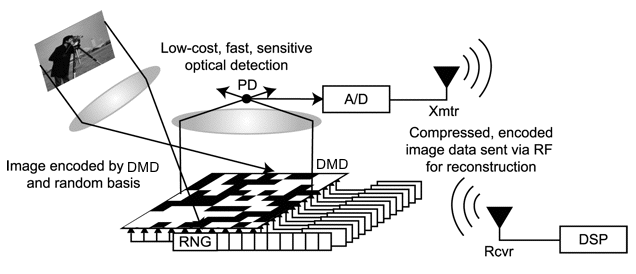
\includegraphics[width=\textwidth]{rysunki/cscam.png}
\caption{Schemat jednopikselowej kamery}
\label{fig:singlePixelSchema}
\end{figure}

\begin{figure}
\centering
	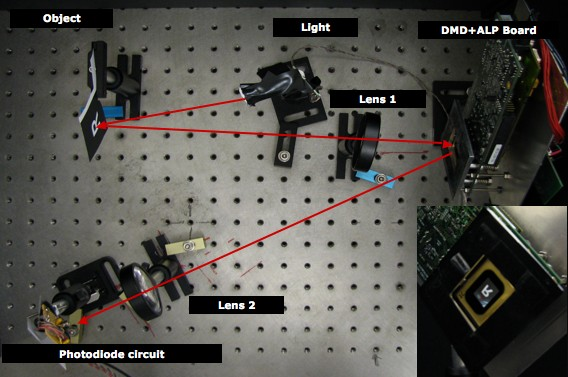
\includegraphics[width=0.6\textwidth]{rysunki/cscamerasetup.jpg}
\caption{Zestawienie jednopikselowej kamery na stanowisku laboratoryjnym}
\label{fig:singlePixelSetup}
\end{figure}

Jednopikselowa kamera to prototyp urządzenia pomiarowego, skonstruowany przez naukowców uniwersytetu RICE \cite{SinglePixelCamera}. Składa się ona z~jednej fotodiody ("piksela"), dwóch soczewek i~matrycy mikroluster (ang. \textbf{DMD} - \textit{Digital Micromirror Device}) \ref{fig:singlePixelSetup}. Ustawienie luster macierzy jest sterowane komputerowo. Podanie 1 na poszczególny element DMD powoduje jego skierowanie w~kierunku drugiej soczewki, zaś 0 - z~dala od niej. Wartości między 0 a~1 mogą być uzyskane przez wielokrotne sterowanie elementem matrycy w~czasie całkowania sygnału na odbiorniku. Zgromadzone na fotodiodzie napięcie jest konwertowane do postaci cyfrowej i~wysyłane drogą radiową do odbiornika \ref{fig:singlePixelSchema}. Ze względu na długi proces pomiarowy, trudno wyobrazić sobie, by powyższa konstrukcja była w~stanie wyprzeć zwykłe kamery w~codziennych zastosowaniach. Może jednak stanowić atrakcyjną cenowo alternatywę dla czujników światła w~zakresach niewidzialnych dla oka.

\subsubsection{Formalne sformułowanie problemu}
W swym doskonałym artykule \cite{CandesIntro} Emmanuel Candes, jeden z~pionierów dziedziny przetwarzania rzadkiego, przedstawił podstawowe obserwacje naukowców umożliwiające zastosowanie metody, dokonał pewnych oszacowań ilościowych, dotyczących potrzebnej liczby pomiarów i~ograniczeń metody na dzisiejszym etapie rozwoju.
Dziedzina przetwarzania rzadkiego wykorzystuje fakt \textit{rzadkości} sygnału oraz \textit{niekoherencji} \cite{Candes2006} różnych baz przestrzeni liniowych. Pierwsze z~pojęć oznacza możliwość przechowania większości użytecznych informacji o~sygnale w~niewielkim obszarze danych. Ściślej rzecz biorąc, reprezentacja $x = \phi \alpha$ w~bazie $\phi$ jest k-rzadka, gdy $K \ll N$ współczynników $\alpha$ dokładnie opisuje $x$. Niekoherencja wyraża z~kolei ideę, że mając rzadką reprezentację sygnału w~jednej bazie, jest ona znacznie rozłożona w~innej. Przykładem może być delta Diraca, która choć w~dziedzinie jest reprezentowana przez jeden pik, jest funkcją stałą w~całej dziedzinie częstotliwości. Wykorzystując dwie powyższe obserwacje, można skonstruować taki sposób pomiaru, który próbkuje go od razu w~skompresowanej formie, bez potrzeby jego zrozumienia. 

Przyjmujemy, że informacja o~sygnale $f_t$ jest uzyskiwana poprzez liniowe funkcjonały
\begin{equation}
	y_k = <f, \varphi_k>, k = 1,...,m.
\end{equation}
Gdzie $\varphi_k$ wyraża sposób pomiaru. Przykładowo, dla matrycy CCD będzie to funkcja charakterystyczna jej danego piksela, a~dla rezonansu magnetycznego - sinusoida o~określonej częstotliwości.

Sposób wykonania m pomiarów przechowujemy w~macierzy pomiarowej $A \in R^{M*N}$. Tym samym, problem CS może zostać opisany jako nieoznaczone równanie liniowe: 
\begin{equation}
	y = A \cdot x
	\label{eq:lin}
\end{equation}

Powyższe równanie posiada nieskończoną liczbę rozwiązań z~$N - M$ stopniami swobody. Rekonstrukcja $x$ polega na takim wybraniu rozwiązania, które najlepiej spełnia postawione przed nim dodatkowe założenia. Najbardziej oczywistym jest znaleźć najrzadsze rozwiązanie, tzn.
\begin{equation}
	\hat{x} = \argmin_z \|x_0\| \text{spełniający} \Phi x=y
	\label{eq:l0}
\end{equation} \cite{CandesIntro, Davenport2010, Zhang2013}, gdzie $\|x\|_0$ = ilość niezerowych współczynników x. Użycie normy zero cechuje się jednak kombinatoryczną złożonością obliczeniową i nie jest realizowalne w dużej skali. Najczęściej jednak udaje się dokładnie odzyskać rzadki sygnał, rozwiązując problem prostego dopasowania (\textbf{BP} - \textit{basis pursuit}):
\begin{equation}
\min_{x \in R^n} \|x_1\| 
\label{eq:l1}
\end{equation}, gdzie $\|x\|_1 = \sum_{i=1}^{n} |x_i|$. Problem \ref{eq:l1} ma wyraźną przewagę nad \ref{eq:l0}, gdyż daje się rozwiązać metodami programowania liniowego \cite{Fountoulakis2012}. Część algorytmów odtwarzania sygnałów rozwiązuje zmodyfikowaną wersję \ref{eq:l1}. Istnieje również wiele metod rekonstrukcji sygnału, wykorzystując algorytmy zachłanne, stochastyczne lub wariacyjne.
 
Warto przy tej okazji wspomnieć, że przetwarzanie rzadkie wykorzystywane jest także dla sygnałów ciągłych \cite{Eldar2009}, zaszumionych i~nie całkowicie rzadkich \cite{Cevher2009}. W~takim wypadku $\alpha$ stanowi aproksymację $x$. Jak pokazują wyniki rekonstrukcji zdjęć, są one wciąż bardzo skuteczne. 
\newline{}
Istotnym osiągnięciem CS jest jego zdolność do oszacowania liczby pomiarów tak, by rekonstrukcja przebiegła pomyślnie z~prawdopodobieństwem bliskim pewności \cite{CandesIntro}. Jest ona zależna od rzadkości reprezentacji sygnału w~danej bazie oraz niekoherencji bazy, w~której próbkujemy sygnał z~bazą rozrzedzającą $x$. Wielkość tę definiujemy następująco:
\begin{equation}
	\mu (\Phi,\Psi) = \sqrt{n} \max_{i, j} |<\phi_i, \psi_j>|
	\label{eq:coherence}
\end{equation}
Okazuje się, że bezpiecznym wyborem jest losowe próbkowanie sygnału, gdyż jest ono niekoherentne z~dowolną, ustaloną bazą $\phi$. Pozostaje więc odpowiednio dobrać sposób jego reprezentacji.

\subsection{Zarys proponowanego rozwiązania}
Rozwiązanie problemu CS wymaga podjęcia kilku kluczowych decyzji. Po pierwsze, należy starannie wybrać sposób próbkowania sygnału, bazę, w~której będzie on reprezentowany oraz algorytm jego rekonstrukcji. W~rozważaniach należy również wziąć pod uwagę docelową architekturę sprzętową i~jej możliwie pełne wykorzystanie.
\subsubsection{Wybór macierzy pomiarowej}
Punktem wyjścia w~badaniach był pakiet $\ell_1$-magic \cite{SinglePixelCameraCode}, zawierający kod źródłowy wybranych algorytmów odtwarzania sygnałów oraz dokument \cite{L1MagicNotes}  je opisujący. Pierwszym ważnym wnioskiem płynącym z~publikacji jest konieczność wyrażenia macierzy pomiarowej w~sposób ukryty, nie wymagający jawnego przechowywania w~pamięci. Jej wielkość bardzo szybko urasta bowiem do ogromnych rozmiarów. Dla przykładu, macierz pomiarowa eksperymentu, w~którym dokonano 20 \% pomiarów zdjęcia o~wielkości 256x256 pikseli, zapisana w~formacie \textit{float} będzie zajmować ponad 3GB pamięci, stanowczo za dużo, zmieścić ją w~RAM GPU.~Powyższy wniosek stanowi to problem z~dwóch powodów. Po pierwsze, jak w~skompresowany sposób zapisać losowe ciągi liczb wysyłane do DMD? Po drugie, zastosowanie implikowanej formy macierzy znacznie utrudnia przyspieszenie obliczeń za pomocą karty graficznej. Nie próbując jednak od razu odpowiedzieć na wszystkie stawiane wyzwania, rozpoczęto badania bogatej literatury CS.~We wstępie \cite{Fountoulakis2012} dostępny jest imponujący przegląd dostępnych metod próbkowania i~odzyskiwania sygnału. Oprócz braku konieczności przechowywania macierzy pomiarowej w~pamięci, autor narzuca ciekawe ograniczenie - możliwie szybkie mnożenie macierzy z~wektorem (np. $\mathcal{O}(nlog(n))$ lub $\mathcal{O}(n)$).  Przyspieszenie tej operacji znacząco skróci czas odtwarzania sygnału, bez względu na wykorzystaną architekturę sprzętową. 
\newline{}
Ciekawą propozycją autorów jest niepełna macierz Fouriera. Jej konstrukcja polega na losowym wybraniu m rzędów macierzy Fouriera o~rozmiarze n x n. Nie wymaga przechowywania w~pamięci, a~jej iloczyn z~wektorem daje się szybko obliczyć wykorzystując algorytm FFT (cechuje się on złożonością $\mathcal{O}(nlog(n))$). Niestety, jej postać spełnia \ref{eq:l1} z~ogromnym prawdopodobieństwem dla znacznie większej liczby pomiarów niż wykorzystując zwykłą macierz losową o~rozkładzie Gaussa  \cite{Rudelson2008}. Postanowiono więc poszukać innych rozwiązań. W swym doskonałym artykule \cite{Peyre2010}, Gabriel Peyre ocenia kilka ortonormalnych baz, które mogą posłużyć jako sposoby rzadkiej reprezentacji sygnału. W praktyce zdjęcia są skutecznie rozrzedzane przez bazę falkową, kosinusową czy curvelet \cite{CurveletWebSite, Candes2000}. Według autora, każda z powyższych posiada swe wady i zalety, zatem aby móc odtwarzać sygnał o różnej charakterystyce, bazę reprezentacji należy dobierać dynamicznie. Jest to niewątpliwie ciekawe podejście, ale wymagające ogromnego nakładu pracy i zostało porzucone. Z tego samego powodu porzucono również ideę poszukiwania najrzadszej bazy sygnału poprzez estymację macierzy $Q$ transformacji Karhunena-Loeve'a \cite{Gwon2012}. \footnote{Odzyskujemy $s = Q^H x$, gdzie $R_x = E[xx^H]$ i $R_x = Q \Lambda Q^H$. Kolumny $Q$ to wektory własne $R_x$, $\Lambda$ to diagonalna macierz wartości własnych.} Zainteresowało nas jednak próbkowanie sygnału za pomocą podmacierzy bazy Hadamarda-Walsha. Jej definicja jest prosta \footnote{$W_0$ = 1, $W_j = \frac{1}{\sqrt{2}} \begin{Bmatrix} W_{j-1} & W_{j-1} \\ W_{j-1} & -W_{j-1} \end{Bmatrix}$}, a będąc mocno związaną z bazą Fouriera, pozwala na mnożenie wektorów ze złożonością $\mathcal{O}(nlog(n))$. Ten sam pomysł, choć w bardziej przejrzysty sposób, przedstawiono również w \cite{Davenport2010} i w ramach praktycznego przykładu odniesiono go do jednopikselowej kamery. Macierz pomiarową możemy generować poprzez 
\begin{equation}
	\Phi = \left(\frac{1}{2} \sqrt{N} I_\Gamma W_B + \frac{1}{2} \right) D
\end{equation}
Gdzie $I_\Gamma$ oznacza identycznościową podmacierz $M x N$, uzyskaną przez losowy wybór $M$ wierszy, tak, by $I_\Gamma W_B$ była podmacierzą $W_B$ indeksowaną przez $\Gamma$. Ponadto, $D$ oznacza losową macierz permutacji o rozmiarze $N x N$. Wyrażenie $\frac{1}{2} \sqrt{N} I_\Gamma W_B + \frac{1}{2}$ przeskalowuje elementy macierzy $\Phi$ tak, by mieściły się w zakresie $(0,1)$. Metoda generowania pomiarów wygląda na bardzo atrakcyjną. Niestety, algorytm szybkiego mnożenia macierzy $W_B$ istnieje tylko dla rozmiarów $2^N$. Ponadto, wynik pomiarów sygnału wyrażonego w bazie falkowej $\Phi \Psi$ nie daje teoretycznych gwarancji odtworzenia $x$ z ogromnym prawdopodobieństwem (choć przedstawiona metoda w praktyce daje dobre, powtarzalne rezultaty). Z tego powodu postanowiono poszukać innego rozwiązania. W ciekawym artykule naukowców z uniwersytetu RICE \cite{Baraniuk2010} opisano możliwość założenia pewnej struktury sygnału, co ogranicza przestrzeń rozwiązań, a co za tym idzie - zmniejsza liczbę potrzebnych pomiarów i złożoność obliczeniową algorytmów. Dodatkowo, posiadanie pewnych założeń co do odzyskiwanych danych ułatwia rozróżnienie ich od szumu, co zwiększa stabilność procesu. Niestety, autorzy pracy nie zaproponowali takiego rozwiązania, które z jednej strony znacznie ułatwiałaby odzyskanie sygnału, a z drugiej - było dostatecznie elastyczne. 

Ostatecznie, naszym wyborem stała się rzadka macierz pomiarowa, opisana w \cite{Berinde2008}. Cechuje ją niezwykła prostota. W każdej kolumnie macierzy $A$ wybieramy $d$ jedynek. Dbamy przy tym, by żadne dwa wektory kolumnowe nie były identyczne (co przy $d \ll N$ jest praktycznie niemożliwe). Zaletą tego rozwiązania jest udowodniona odporność na szum, efektywne mnożenie macierzy (wymaga ono nie więcej niż $nd$ dodawań) i niewielka ilość zajmowanego miejsca w pamięci. Przedstawione wyniki empiryczne dla zdjęć o rozmiarze 256x256 potwierdziły, że wykorzystując tę macierz pomiarową, można rozwiązywać problemy w odpowiednio dużej skali. Po decyzji związanej z macierzą pomiarową, przystąpiono do wyboru algorytmu rekonstrukcji zdjęcia.

\subsubsection{Dobór algorytmu rekonstrukcyjnego}
Odpowiedni dobór algorytmu odtworzenia sygnału ma niebagatelne znaczenie na szybkość, stabilność i dokładność procesu. Wyzwaniem stało się odpowiednie dobranie metody dla implementacji na karcie graficznej. Temat ten jest bowiem rzadko podejmowany w publikacjach naukowych. Natrafiono jedynie na jedną bibliotekę implementującą algorytmy odtwarzania sygnału z użyciem kart graficznych \cite{GAGA}. Grupa metod tam wykorzystanych nosi miano zachłannych. Przykładowo, algorytm iteracyjnego progowania (ang. \textbf{IHT} -- \textit{Iterative hard thresholding}) \cite{Blumensath2009} opisany jest następującą, iteracyjną formułą: 
\begin{equation}
\begin{split}
    x_0 & = 0 \\ 
x_{n+1} & = H_s \left(x_n + \Phi^T(y - \Phi x_n) \right)
\end{split}
\end{equation}
\newline{}
Gdzie $H_s(a)$ zeruje wszystkie poza $s$ największymi współczynniki $x$. Algorytm cechuje niezwykła prostota. Jedna jego iteracja wymaga dwóch mnożeń macierz-wektor i częściowego posortowania elementów $a_n =  H_s \left(x_n + \Phi^T(y - \Phi x_n) \right)$. Łatwo wyobrazić sobie równoległą implementację takiego rozwiązania, np. przy użyciu algorytmu \textit{mergesort} \cite{Thouti2012}. Dodatkową zaletą rozwiązania jest niewielka ilość przechowywanych danych. Niestety, prostota i szybkość algorytmu odbija się na jego dokładności. W kontekście zdjęć ich wyjście może stanowić pierwsze przybliżenie rozwiązania problemu \ref{eq:l1}. W szczególności, metody zachłanne słabo aproksymują niezbyt rzadki sygnał ($\frac{k}{n} \ge 0.2$, gdzie $k$ - liczba znaczących elementów $x$, $n$ - rozmiar $x$). Z tego powodu zrezygnowano z tej klasy algorytmów i zwrócono się w stronę klasycznych metod optymalizacyjnych rozwiązujących problem \ref{eq:l1} lub pokrewny.

Ponownie, punktem wyjścia w naszych rozważaniach były algorytmy zaimplementowane w pakiecie $\ell 1$-MAGIC \cite{SinglePixelCameraCode}. Grupa metod programowania liniowego minimalizujących normę $\ell 1$ okazały się jednak skutecznie głównie dla sygnałów prawdziwie rzadkich. Odtworzenie zdjęcia algorytmem $\ell 1$-pd \cite{Boyd2004} w aplikacji współtworzonej przez jednego autorów projektu \cite{PR12SIS306} było skuteczne, gdy $\frac{m}{n} \ge  0.6$. Chcąc znacząco poprawić ten wynik, należało poszukać innej metody rozwiązania. Pamiętając również o akceleracji obliczeń przy pomocy karty graficznej, przyglądnięto się klasie algorytmów zwykle implementowanych na tych urządzeniach. 

Za niezwykle interesujący uznano algorytm \textbf{TVQC} \cite{Candes2005a,Candes2005b}. Rozwiązuje on następujący problem optymalizacyjny:
\begin{equation}
\begin{split}
& \min_{TV} ~~\text{spełniający}~~\|Ax - y \|_{\ell 2} \le \epsilon \\
\text{gdzie:} &\\
              & \|x \|_{TV} = \sum_{i,j} \sqrt{ \left( x_{i+1,j} - x_{i,j} \right)^2 + \left( x_{i,j+1} - x_{i,j} \right) ^2} = \sum_{i,j}|\left(\nabla x \right)_{i,j} |
\label{eq:TV}
\end{split}
\end{equation}

Podstawowym założeniem tej metody jest rzadkość (lub kompresowalność) \textit{gradientu} zdjęcia. Jest ono słuszne dla dużej części naturalnych ekspozycji i tylko nieznacznie zmniejsza uniwersalność metody. Baza gradientu sygnału wydaje się być wysoce niekoherentna z rzadką macierzą pomiarową. Dokonano bowiem udanych rekonstrukcji zdjęć przy użyciu ok. 8\% pomiarów \cite{Berinde2008}. Jedyną zagadką pozostała ocena wydajności algorytmu zaimplementowanego na karcie graficznej. Nie odnaleziono bowiem żadnych prób równoległej implementacji algorytmu. Postanowiono jednak podjąć próbę i wyciągnąć odpowiednie wnioski z przeprowadzonych testów.
